\documentclass{standalone}
\usepackage{tikz}
\usetikzlibrary{shapes.symbols, positioning}

\begin{document}
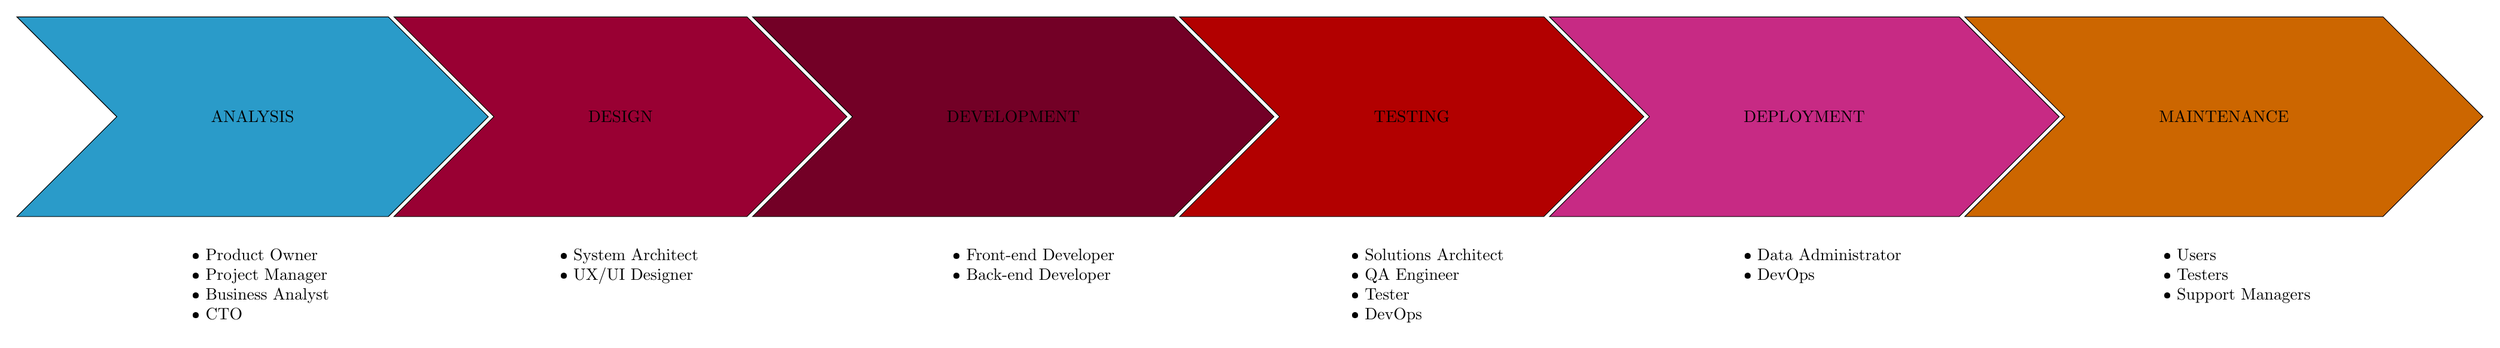
\begin{tikzpicture}

% Define styles
\tikzstyle{role} = [text width=3cm, align=left, below]

\tikzset{
    phase/.style={
        draw,
        signal,
        signal to=east,
        signal from=west,
        inner sep=2cm,
    }
}


% Define the phases
\node[phase, fill=cyan!80!black] (analysis) {ANALYSIS};
\node[phase, fill=purple!80!black, right=0.1cm of analysis] (design) {DESIGN};
\node[phase, fill=purple!60!black, right=0.1cm of design] (development) {DEVELOPMENT};
\node[phase, fill=red!70!black, right=0.1cm of development] (testing) {TESTING};
\node[phase, fill=magenta!80!black, right=0.1cm of testing] (deployment) {DEPLOYMENT};
\node[phase, fill=orange!80!black, right=0.1cm of deployment] (maintenance) {MAINTENANCE};

% Define the roles for each phase
\node[role, below=0.5cm of analysis] {
  \begin{tabular}{l}
  \textbullet\ Product Owner \\
  \textbullet\ Project Manager \\
  \textbullet\ Business Analyst \\
  \textbullet\ CTO
  \end{tabular}
};

\node[role, below=0.5cm of design] {
  \begin{tabular}{l}
  \textbullet\ System Architect \\
  \textbullet\ UX/UI Designer
  \end{tabular}
};

\node[role, below=0.5cm of development] {
  \begin{tabular}{l}
  \textbullet\ Front-end Developer \\
  \textbullet\ Back-end Developer
  \end{tabular}
};

\node[role, below=0.5cm of testing] {
  \begin{tabular}{l}
  \textbullet\ Solutions Architect \\
  \textbullet\ QA Engineer \\
  \textbullet\ Tester \\
  \textbullet\ DevOps
  \end{tabular}
};

\node[role, below=0.5cm of deployment] {
  \begin{tabular}{l}
  \textbullet\ Data Administrator \\
  \textbullet\ DevOps
  \end{tabular}
};

\node[role, below=0.5cm of maintenance] {
  \begin{tabular}{l}
  \textbullet\ Users \\
  \textbullet\ Testers \\
  \textbullet\ Support Managers
  \end{tabular}
};

\end{tikzpicture}
\end{document}
